\chapter{\agentj: The Toolkit}
\label{agentj}

The chapter provides a brief snapshot of the AgentJ toolkit. It provides an overview of the AgentJ source tree, followed by a high-level overview of the software architecture. We then provide an explanation of what is required in order to create a Java Ns-2 Agent for AgentJ.  

\index{AgentJ Ns-2 Agents}

\section{A Root Around the AgentJ Directories}
\label{agentj:classes}

\index{AgentJ directory structure}

\begin{figure}
\centering
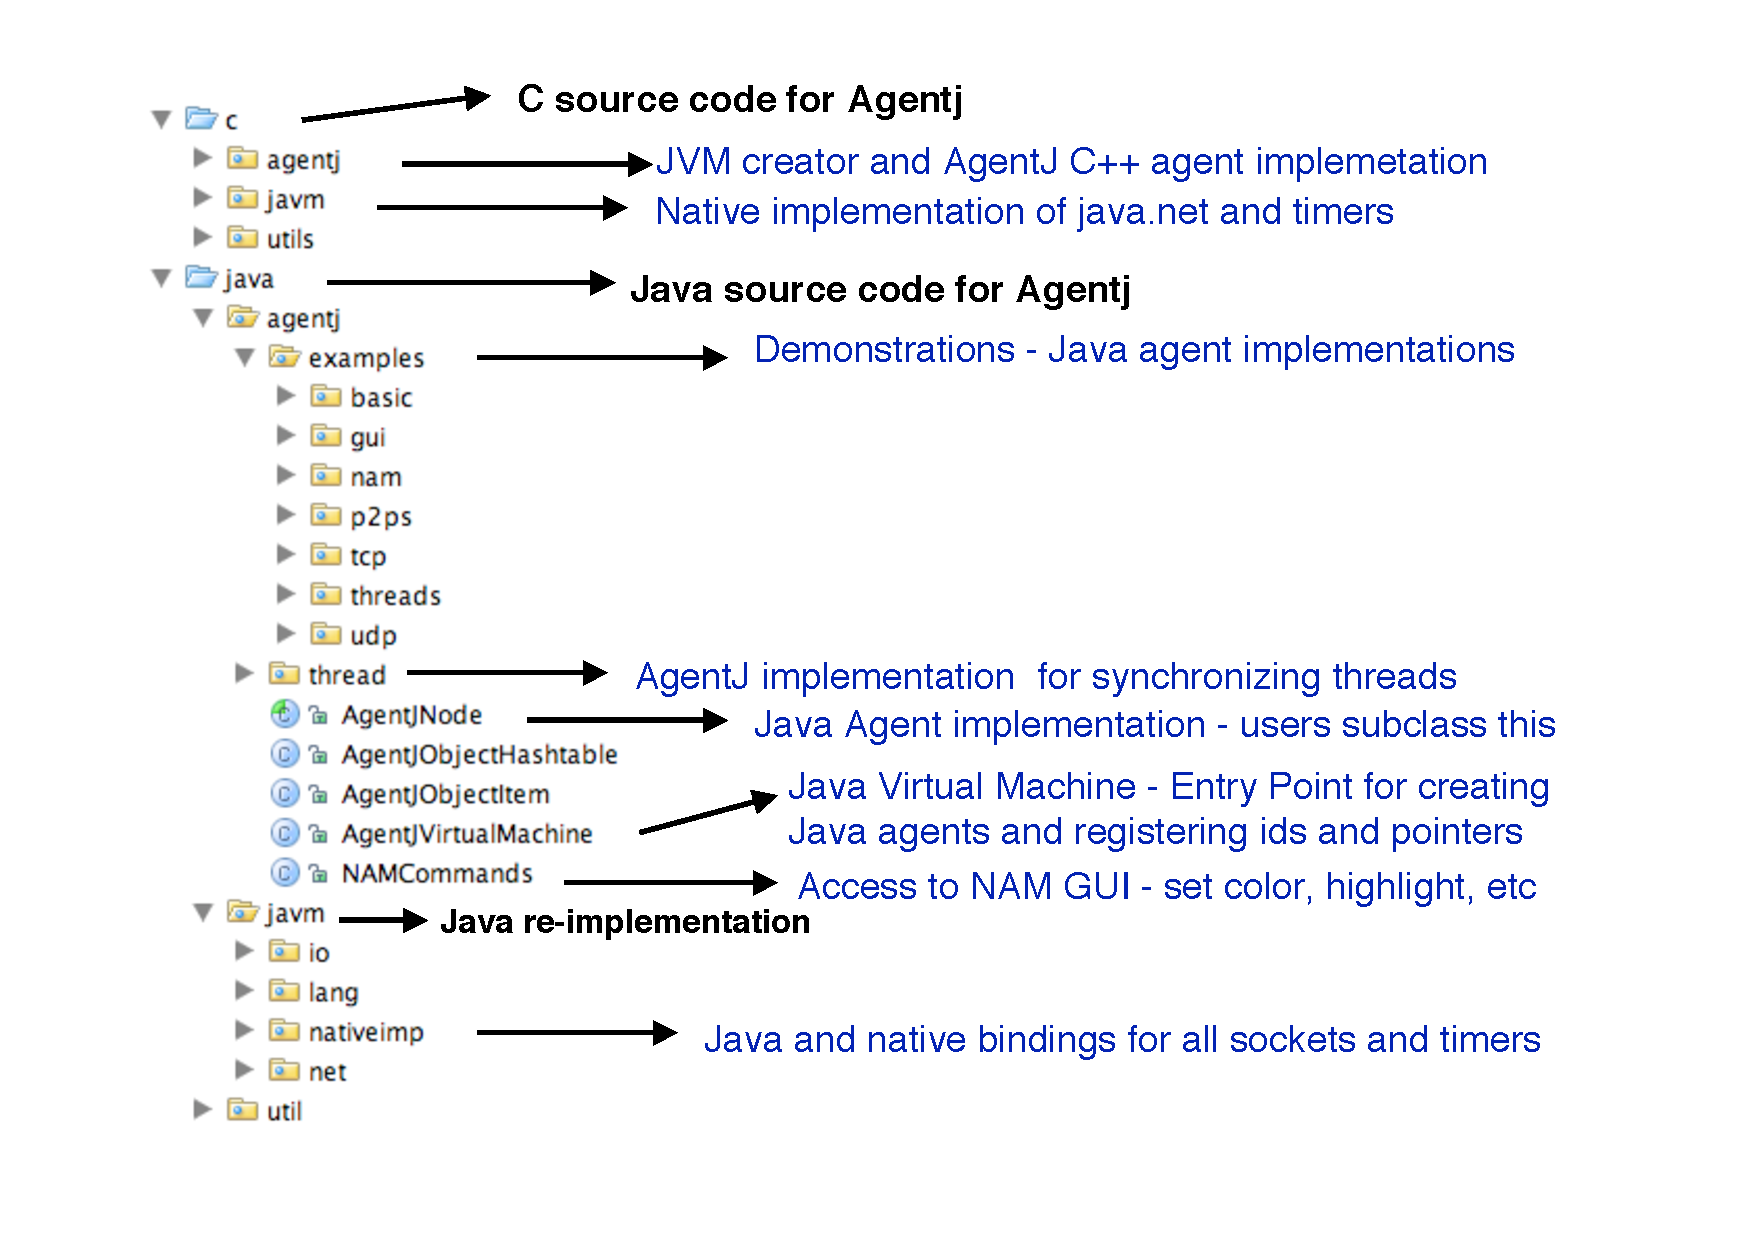
\includegraphics[scale=0.50]{images/directories}
\caption{The C++ Classes within \agentj.}
\label{fig:directories}
\end{figure}

\agentj~is made up of a collection of C++ and Java classes.  The \agentj~directorty 
tree is organized as if it was a Java application.  Therefore,
within this \agentj~directory, there is a classes directory (where all classes
live), a lib directory (for JAR files plus native shared libraries), a doc directory
(containing this manual) and a src directory (for all source files), amongst
others.

\index{C++ clases}

The src directory has a java and c subdirectory containing the Java and native
code, respectively as shown in Figure \ref{fig:directories}.  In the C directory there are three directories: agentj, javm and utils.  The \emph{agentj} directory contains the 
Ns-2 agent code (AgentJ.cpp) that implements the core Ns-2 agent capabilities for 
spawning the AgentJ software and tools. This class instantiates a \emph{AgentjVirtualMachine} object, also contained in this directory, upon first creation, which creates a Java virtual machine for interacting with the Java codes.  It thereafter passes commands via the \emph{AgentjVirtualMachine} class to be passed to the Java objects (using a pointer to the Ns-2 C++ agent for identification). The \emph{javm} directory contains the classes for the implementation of the Java native interface Java Virtual Machine (JAVM), which bind to the underlying Protolib classes for implementation for integration into Ns-2.  

\index{Java classes}

In the Java directory, we have the corresponding \emph{javm} directory that contains the Java side of the AgentJ implementation of \emph{java.net}, \emph{java.io} and some \emph{java.lang} clases.  It also contains the reciprocal of the C++ AgentjVirtualMachine class, called AgentJVirtualMachine.java, which contains the entry point static methods called by the C++ class and the \emph{AgentJNode.java} class which is the abstract base class implementation of any Java NS-2 agent implemented by a user. In the root directory, there is also a NAMCommands class that allows you to annotate messages and colors onto your NAM visualisation during execution. There is an \emph{examples} directory, which is covered in chapter \ref{chap:examples} and a \emph{thread} directory which contains the Java code for thread synchronisation and the monitoring of threads during execution. 

\index{P2PS}

\section{From the Java Side to the C Side}

Since AgentJ is a Java environment for Ns-2, a JNI bridge is needed in 
order to map between the C++ NS2 agents and the associated Java 
agents. This bridging mechanism is required at both the input to
the Java initialisation and at its lower communication layers; that is, 
first the C++ NS-2 agents need to instantiate and attach Java 
agents to the NS-2 C++ agents, then the Java agents need to be able to
access the Protolib interface in order to pass data between themselves in NS-2.
In the first case, a C++ environment creates a Java Virtual Machine 
(JVM) (using the \emph{AgentjVirtualMachine.cpp} and 
\emph{AgentJVirtualMachine.java} classes) for 
creating and accessing Java objects.  In the second case, we provide a 
mapping from \emph{java.net} to the Protolib C++ libraries 
using JNI.  The resulting interaction is shown 
in Figure \ref{intro:fig:impoverview}.  This figure shows how Java 
is used by NS-2 to create the overall picture.  Each C++ NS2 \emph{agent} 
attaches a Java object (i.e. Java agent) via a call to 
\emph{AgentjVirtualMachine.cpp} which invokes the \emph{attachJavaAgent} 
method in \emph{AgentJVirtualMachine.java} using JNI for registration of 
the agent.  

\index{C++ NS-2 Agent}
\index{Java NS-2 Agent}
\index{AgentjVirtualMachine.cpp}
\index{AgentJVirtualMachine.java}

\begin{figure}
\centering
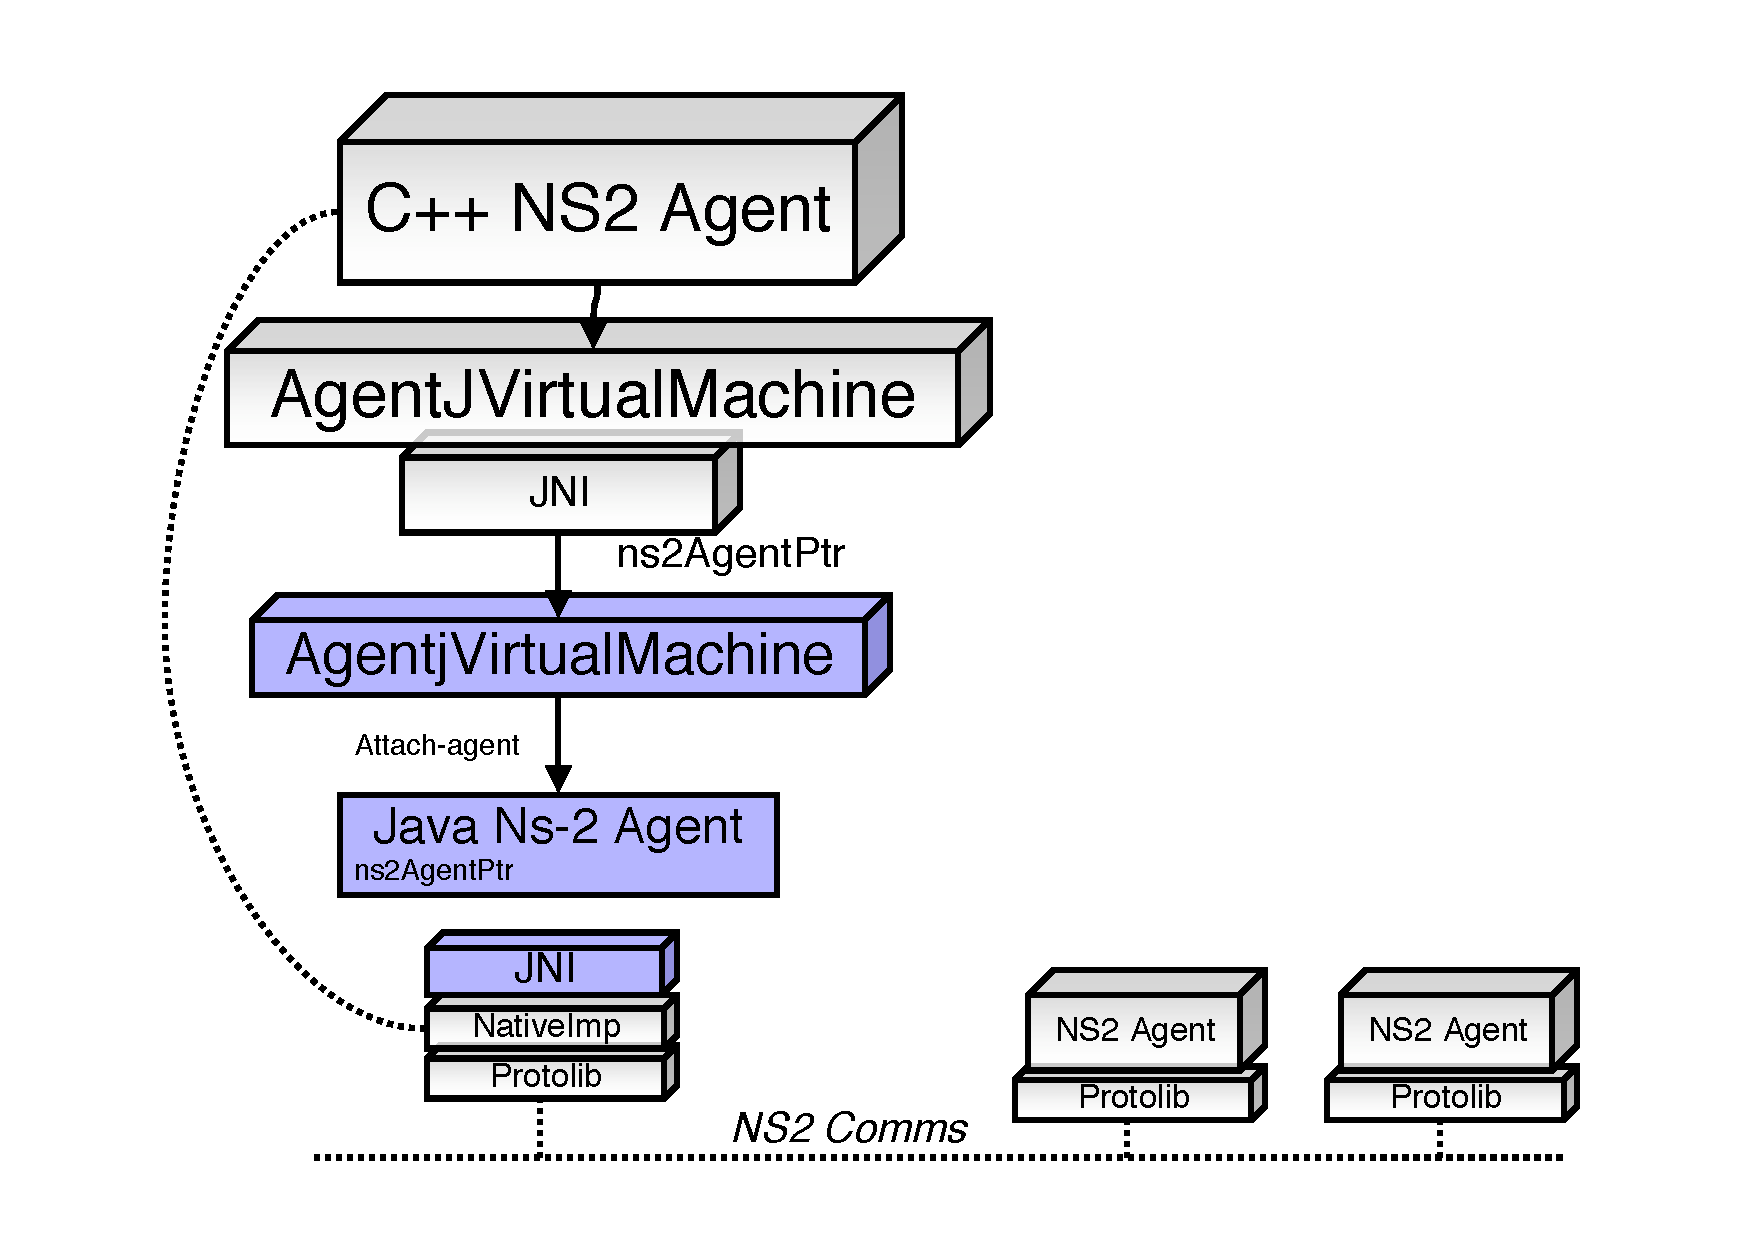
\includegraphics[scale=0.4]{images/impoverview}
\caption{An overview of the \agentj~software components} 
\label{intro:fig:impoverview}
\end{figure}

\index{NS2}
\index{JNI}
\index{Java}
\index{JVM}

There could potentially be thousands of NS2 nodes and each one
might want to instantiate and use a Java object.  Therefore serious
scalability issues can be encountered if this interaction is not
slimline enough. In \agentj, the C++ JVM helper class 
(AgentjVirtualMachine.cpp) therefore only creates one 
JVM per simulation.  The JVM then interfaces through a singleton
\emph{AgentJVirtualMachine.java} class, which creates and manages the 
Java objects. \emph{AgentjVirtualMachine} contains functionality that can
dynamically create a Java object from a textual representation of its
name (e.g. agentj.examples.tcp.SimpleTcp). The registration request
(using \emph{attachJavaAgent}) results in a Java \emph{Hashtable} 
being populated with an item pair; the C++ NS-2 agent pointer representing 
the key and \agentj~Java object representing the object.

\index{JVM Interface}
\index{JNI}

The C++ NS2 agent's \emph{ID} is actually its C++ pointer, which
is reused later within the JNI binding to bind the sockets and timers
onto the Ns-2 agent that issued the command to attach them. 


\section{Sending commands to Java Agents}

\index{Command interface}

 A Java NS2 agent is attached to a C++ NS2 node and is accessed in the
 same way as C++ Ns2 agents are accessed, through the command() interface. 
Thus, specifically, an \agentj~node is:

\emph{
\begin{quote}
A Java object that extends the \emph{AgentJObject} abstract class (and therefore implements the required command() method).
\end{quote}
}

\vspace{0.1in}

Ns-2 Java agents typically provide commands that hook into 
3rd party Java application in order to provide simulation tests for those 
applications. You can think of Ns-2 agents as a replacement to a GUI
or a command line interface that instructions your application to do
certain things at a certain time with respect to the choreography 
of your simulation i.e. to specify what you want to simulate.

 \begin{figure}
 \centering
 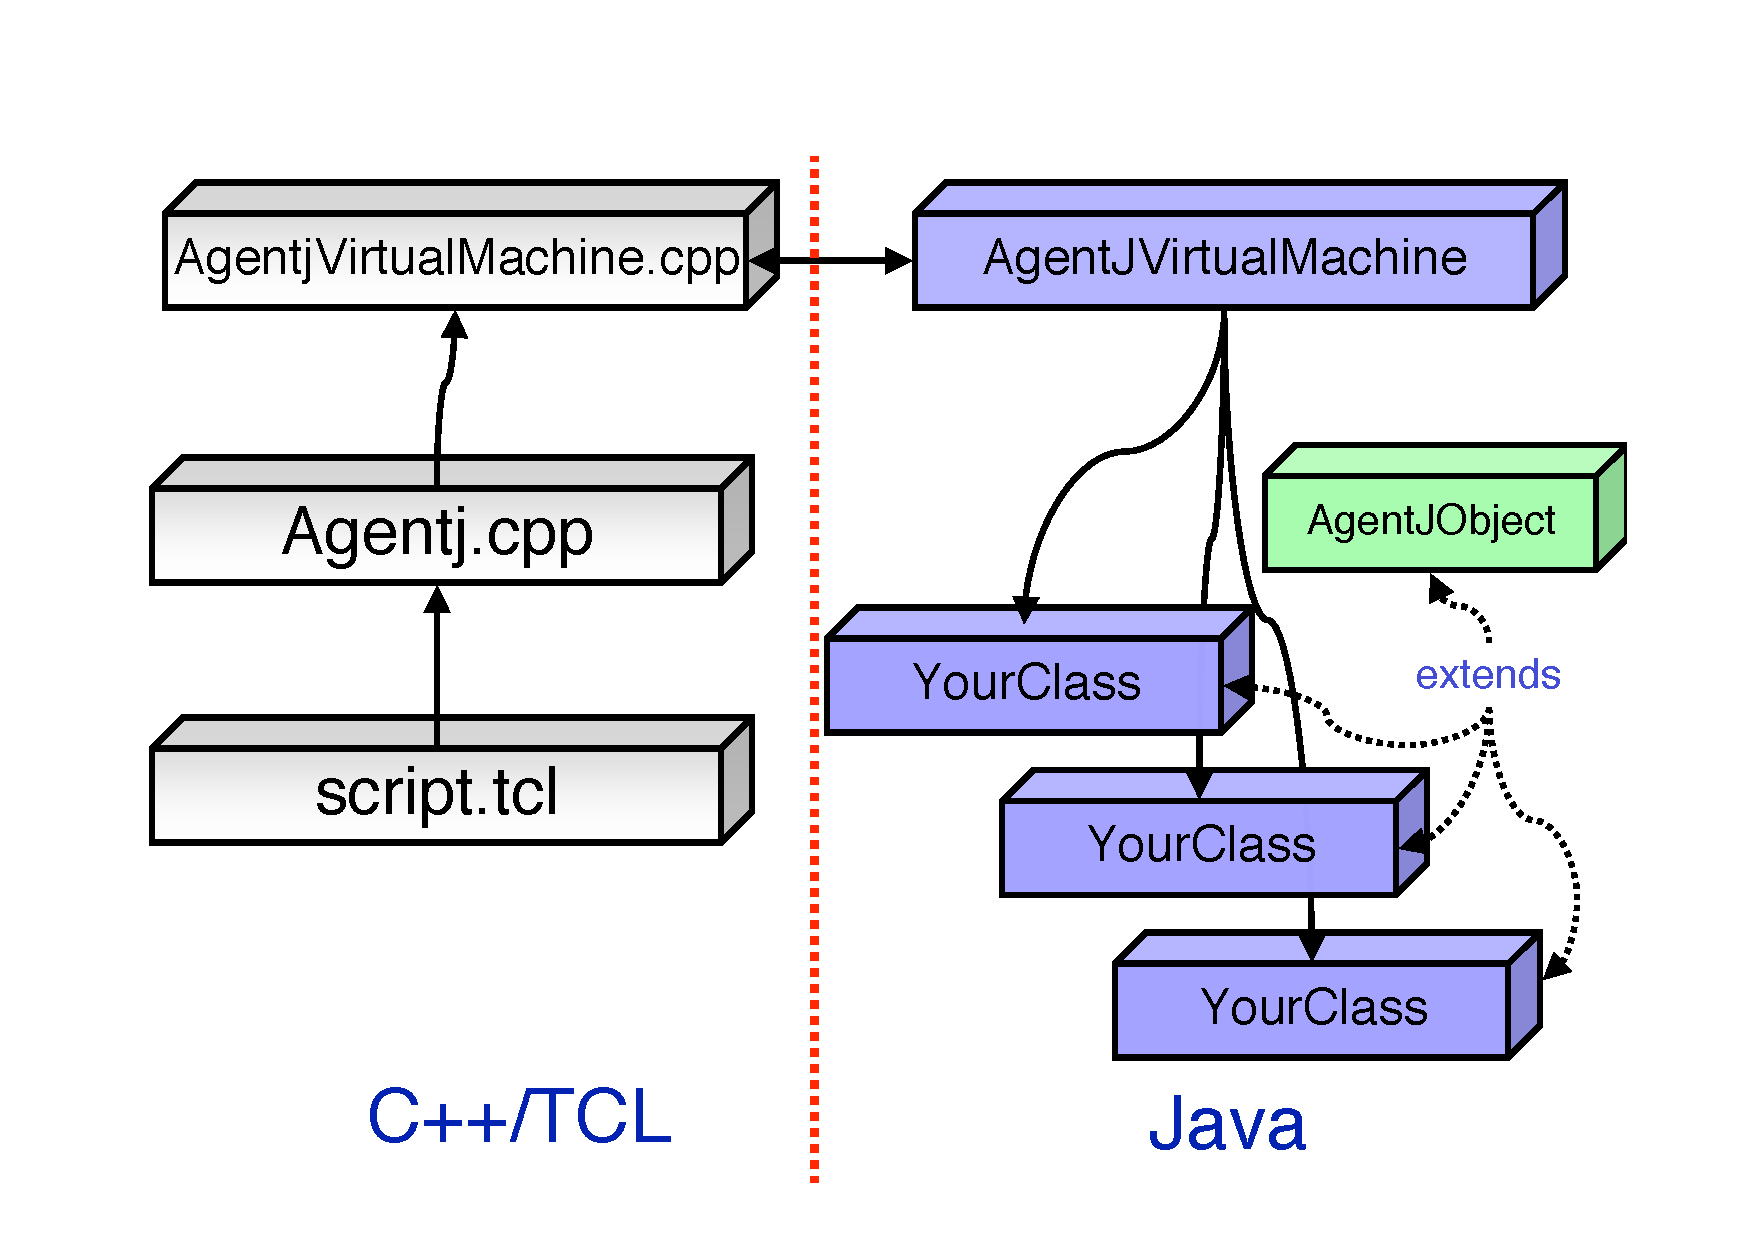
\includegraphics[scale=0.4]{images/progoverview}
 \caption{The interaction between TCL and Java objects through the command() method in AgentJObject. }
 \label{fig:progoverview}
 \end{figure}

\index{TCL simulation script}

Figure \ref{fig:progoverview} shows interaction between the simulation orchestration (in TCL), the C++ agent and its associated Java class.  The programmer who wishes to use
 Java functionality within their NS2 simulations only needs to be
 concerned within their NS2 TCL script and their Java class that
 implements the behaviour they require. The relationship between an Ns2 agent
 and its Java class is very similar to the relationship between an NS2
 TCL script and its associated C++ class (i.e. an NS2 agent) which
 implements the same kind of interaction through sending text
 commands between the two. The Java interface
 employs the same mechanism to bridge these different
 programming languages. The C++ agent (Agentj.cpp) simply acts
 as a go-between to pass commands across to the
 appropriate Java object, via the C++ AgentjVirtualMachine and 
 corresponding AgentJVirtualMachine Java classes.

The command-style interface satisfies some essential AgentJ design conditions:

 \begin{itemize}
 \item  \textbf{Simplicity:} the scalability issues and framework for interacting with
 the Java objects can easily be hidden behind the container C++ and Java classes
 - the programmer does not need to be aware of their presence.
 \item  \textbf{Familiarity:} this mechanism allows communication between the
 NS2 agent and any attached Java class through the same familiar interface as NS2 programmers interface between the TCL scripts and C++ agents now. Users and programmer do not need to learn a new mechanism.
 \end{itemize}

 This interaction is shown in Figure \ref{fig:useroverview}, which illustrates
 the two key commands for attaching and interacting with a Java
 agent from TCL.  Each Ns2 node creates a Java object of its own 
 choice by using the TCL command:

\begin{figure}
 \centering
 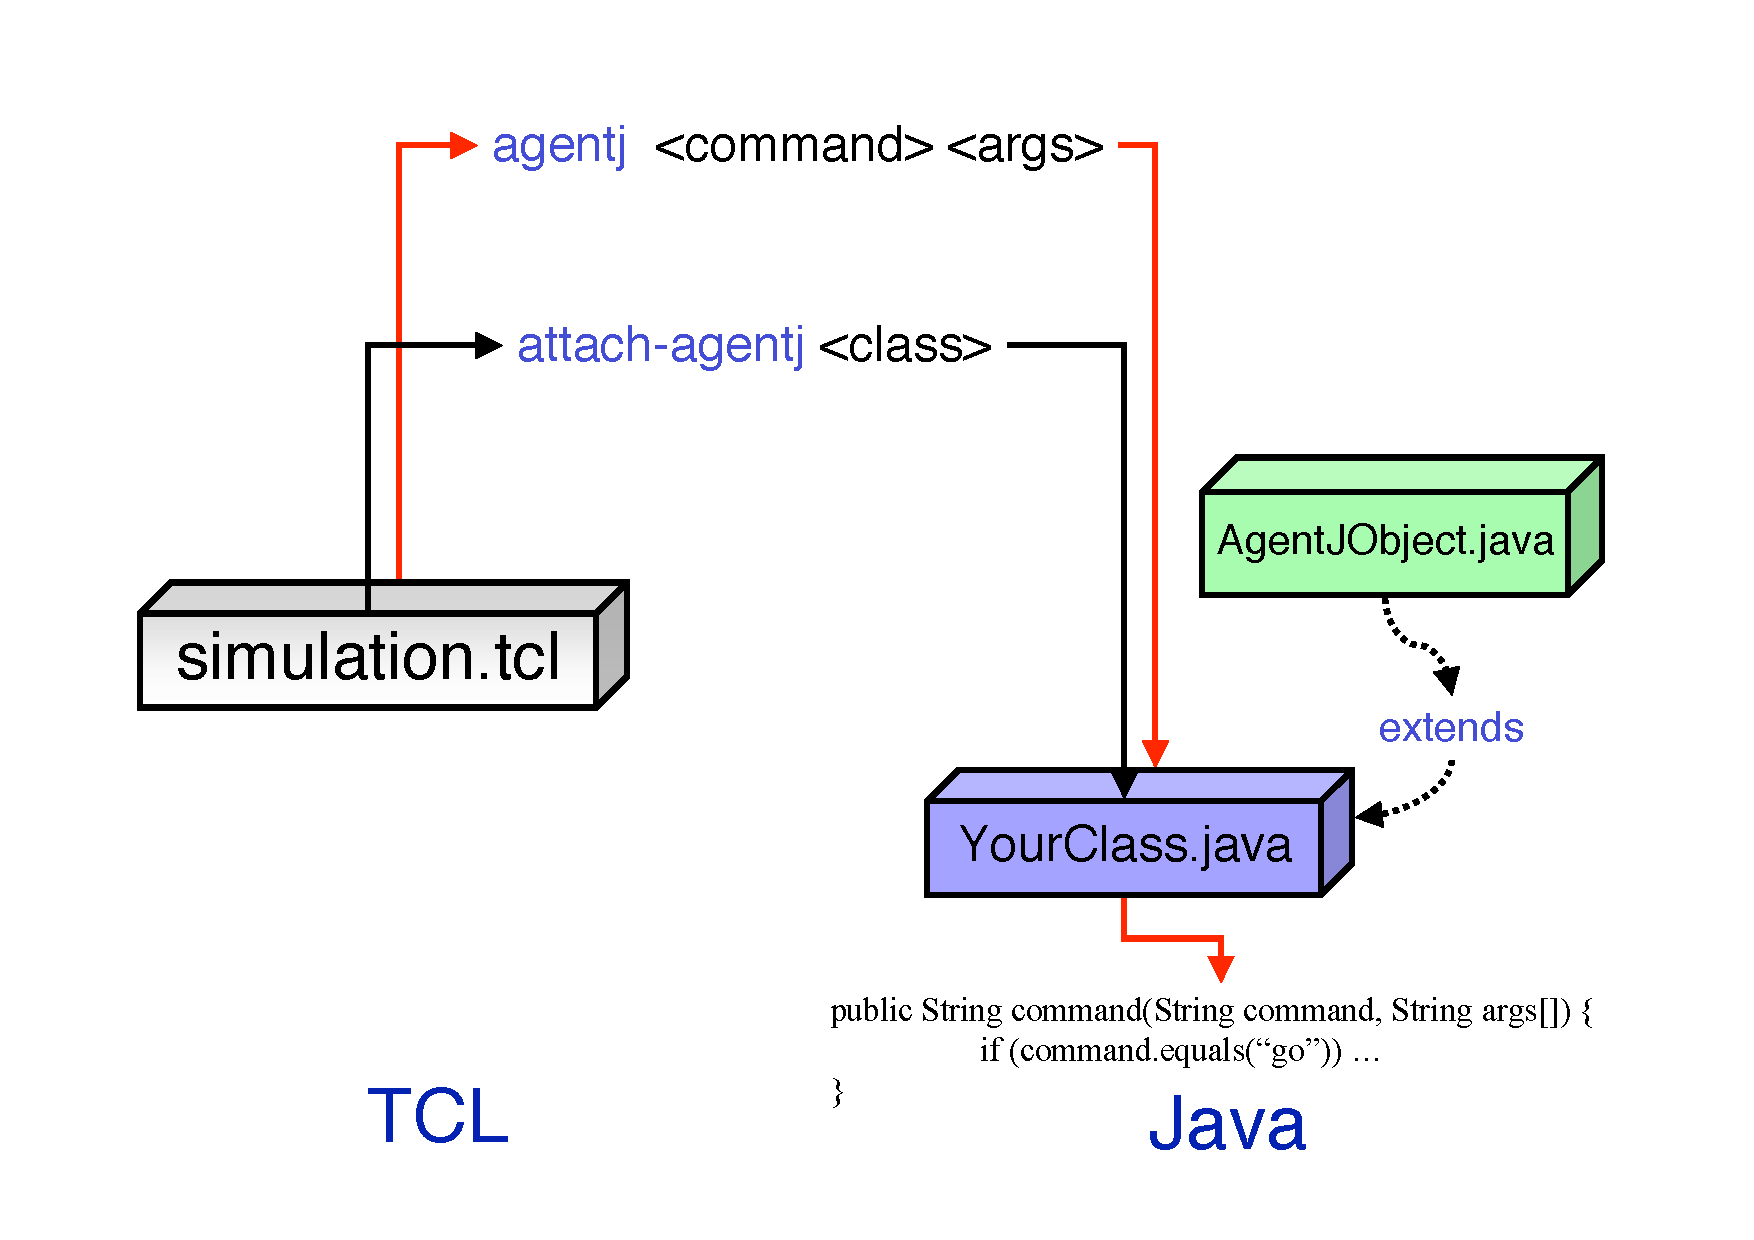
\includegraphics[scale=0.4]{images/useroverview}
 \caption{The interface to a Java program for an agent employs
 a similar interface to that of NS2 when communicating between
 the TCL scripts and the C++ classes. }
 \label{fig:useroverview}
 \end{figure}

 \footnotesize
 \begin{verbatim}
 attach-agentj <class>
 \end{verbatim}
 \normalsize

 \noindent where class can be any fully qualified Java class name.  For example, to attach the ChangeDelimiter class to a node, you would use:
 
  \index{TCL attach-agentj command}

 \footnotesize
 \begin{verbatim}
 attach-agentj agentj.examples.basic.ChangeDelimiter
 \end{verbatim}
 \normalsize
 
 \index{TCL agentj command}

 Once the Java object has been created, commands can be sent by using the TCL command:

 \footnotesize
 \begin{verbatim}
 agentj <command> <args>
 \end{verbatim}
 \normalsize

 \noindent which would invoke the java command with the associated
 arguments. So, to invoke the command ``hello'' on ChangeDelimiter, 
 one would use:
 
 \footnotesize
 \begin{verbatim}
$ns_ at 0.0 "$a1 agentj hello A-String-From-P2" 
 \end{verbatim}
 \normalsize

which would have a corresponding implementation within the ChangeDelimiter object, like the following:

 \footnotesize
 \begin{verbatim}
    public boolean command(String command, String args[]) {
       if (command.equals("hello")) {
            System.out.println("ChangeDelimiter(" + myID + ") has "
                    + args.length + " arguments");
            for (int i=0; i<args.length; ++i) {
                System.out.println("Arg[" + i + "] = " + args[i]);
            }
            return true;
        }
       return false;
    }
 \end{verbatim}
 \normalsize

You can try this example out yourself by running the following:


 \footnotesize
 \begin{verbatim}
cd $AGENTJ/examples/basic/
ns changeDelimiter.tcl
 \end{verbatim}
 \normalsize

which should show a number of set-up commands and have an output ending in:

\footnotesize
\begin{verbatim}
Proto Info: AGENTJ COMMAND: hello, Arguments = A-String-From-P2
changeDelimiter(2) has 4 arguments
Arg[0] = A
Arg[1] = String
Arg[2] = From
Arg[3] = P2
 \end{verbatim}
 \normalsize

This process is demonstrated further in the next chapter where a number of more complex examples are provided.



 
